Separating hyperplane classifiers are procedures that construct linear decision boundaries that
explicitly try to separate the data into different classes as well as possible.\\
\sB{Classifier such as $\left\{ x: \hat{\beta}_{0} + \hat{\beta}_{1}x_{1} + \hat{\beta}_{2}x_{2}
= 0 \right\}$ that compute a linear combination of the input features and return the sign}, were
called \tB{\textit{perceptrons}} in the engineering literature in the late $1950's$

Perceptrons set te foundations for the neural network models.\\
For a surface $L$ defined by the equation: $f(x)=\beta_{0}+\beta^{T}x=0$\\
Some properties:
\begin{enumerate}
	\item $\forall (x_{1}, x_{2})\in L^{2},~\beta^{T}(x_{1}-x_{2})=0$ and hence $\beta^{*}=
		\frac{\beta}{\norm{\beta}}$ is the vector normal to the surface $L$
	\item $\forall x_{0}\in L, \beta^{T}x_{0} = -\beta_{0}$
	\item The signed distance of any point $x$ to $L$ is given by:
		\begin{align*}
			{\beta^{*}}^{T}(x-x_{0}) =& \frac{1}{\norm{\beta}}\left( \beta^{T}x+
			\beta_{0} \right)\\
			=& \frac{1}{\norm{f'(x)}}{f(x)}
		\end{align*}
\end{enumerate}
Hence \sB{$f(x)$ is proportional to the signed distance from $x$ to the hyperplane defined by $f(x)=
0$}
\begin{figure}[H]
	\begin{center}
		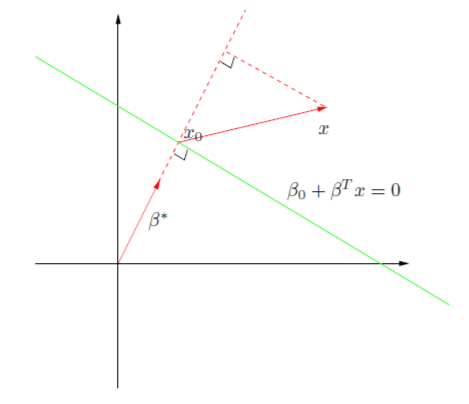
\includegraphics[width=.4\textwidth]{./chap/1chap/3sec/8images/1_hyperplaneAffine.PNG}
	\end{center}
	\caption{The linear algebra of a hyperplane (affine set)}
	\label{fig:1_hyperplaneAffine}
\end{figure}

\paragraph{Rosenblatt's Perceptron Learning Algorithm}
\tB{It tries to find a separating hyperplane by minimizing the distance of misclassified points 
to the decision boundary.} The goal is to minimize: 
%$$ D(\beta, \beta_{0}) = \su{{i\in\mathcal{M}}}{}y_{i}\left(x_{i}^{T}\beta + \beta_{0}\right)$$
\begin{center}
\enc{$D(\beta, \beta_{0}) = \su{{i\in\mathcal{M}}}{}y_{i}\left(x_{i}^{T}\beta + \beta_{0}\right)$}
\end{center}
where $\mathcal{M}$ indexes the set of misclassified points.

\begin{align*}
	\dfrac{\partial D(\beta,\beta_{0})}{\partial\beta}=&-\su{{i\in\mathcal{M}}}{}y_{i}x_{i}\\
	\dfrac{\partial D(\beta,\beta_{0})}{\partial\beta_{0}}=&-\su{{i\in\mathcal{M}}}{}y_{i}\\
\end{align*}
The algorithm in fact uses \tB{\textit{stochastic gradient descent}} to minimize this piecewise 
linear criterion.\\
The misclassified observations are visited in some sequence, and parameters $\beta$ are updated
via:
$${{\beta}\choose{\beta_{0}}} \leftarrow {{\beta}\choose{\beta_{0}}}+\rho {{y_{i}x_{i}}\choose{y_{i}}}$$
$\rho$ is the learning rate.

\paragraph{Optimal Separating Hyperplanes}
The \textit{optimal separating hyperplanes} separates the 2 classes and maximizes the distance
to the closet point from  either class. Consider the optimization problem:
\begin{center}
$\max\limits_{\beta,\beta_{0},\norm{\beta}=1} M$\\
subject to $y_{i}\left(x_{i}^{T}\beta+\beta_{0}\right)\geq M, i\in\inter{1}{N}$
\end{center}
\sB{The set of conditions ensure that all the points are at least a signed distance $M$ from the
decision boundary defined by $\beta$ and $\beta_{0}$}
